Whereas, people have have often tried to categorized objects as GCs by making
cuts along half-light radius, density, and surface brightness profile, in fact
many objects which are generally thought of as GCs don't cleanly fit into these
cuts. Consequently, \citet{Carretta2010} proposed a definition of GC based on
observed chemical inhomogeneities in their stellar populations. The modern
understanding of GCs then is not simply one of a dense cluster of stars which
may have chemical inhomogeneities and multiple populations; rather, it is one
where those chemical inhomogeneities and multiple populations themselves are
the defining element of a GC.

All globular clusters older than 2 Gyr studied in detail show populations
enriched in He, N, and Na while also being deplete in O and C
\citep{Piotto2015,Bastian2018}. These light element abundance patterns also are
not strongly correlated with variations in heavy element abundances. One
consequence of this fact is the spectroscopically uniform Fe abundances
mentioned in \S\ref{sec:intro_GC}. Further, high-resolution spectral studies
reveal anti-correlations between N-C abundances, Na-O abundances, and
potentially Al-Mg \citep{Sneden1992, Gratton2012}. Typical stellar fusion
reactions can deplete core oxygen; however, the observed abundances of Na, Al,
and Mg cannot be explained by the likes of the CNO cycle \citep{Prantzos2007}.

Formation channels for these multiple populations remain a point of debate
amoung astronomers. Most proposed formation channels consist of some older,
more massive, population of stars polluting the pristine cluter media before a
second population forms, now enriched in heavier elements they themselves could
not have generated \citep[for a detailed review see ][]{Gratton2012}. The four
primary candidates for these polluters are asymtotic giant branch stars
\citep[AGBs,][]{Ventura2001,DErcole2010}, fast rotating massive stars
\citep[FRMSs,][]{Decressin2007}, super massive stars
\citep[SMSs,][]{Denissenkov2014}, and massive interacing binaries
\citep[MIBs,][]{deMink2009, Bastian2018}. 

Hot hydrogen burning (proton capture), material transport to the surface, and
material ejection into the intra-cluster media are features of each of these
models and consequently they can all be made to {\it qualitatively} agree with
the observed elemental abundances. However, none of the standard models can
currently account for all specific abundances \citep{Gratton2012}. AGB and FRMS
models are the most promising; however, both models have difficulty reproducing
severe O depletion \citep{Ventura2009,Decressin2007}. Moreover, AGB and FRMS
models require signifigant mass loss ($\sim 90\%$) between cluster formation
and the current epoch --- implying that a signifigant fraction of halo stars
formed in GCs \citep{Renzini2008,DErcole2008,Bastian2015}.

Despite these challenges, predictions of He enhancement distinguishing MPs have
lined up well with isochrone fitting results. Therefore, it is currently
accepted that MPs are primarily parameterized by their Helium abundances
[CITE]. Depending on the cluster, Ys as high as 0.4 have been inferred [CITE].
However, due to the relatively high and tight temperature range of partial
ionization for He it cannot be observed in globular clusters; consequently, the
evidence for enhanced He in GCs originates from comparison of theoretical
stellar isochrones to the observed color-magnitude-diagrams of globular
clusters. Therefore, a careful handling of chemistry is essential when modeling
with the aim of discriminating between MPs; yet, only a very limited number of
GCs have yet been studied with chemically self-consistent (structure and
atmosphere) isochrones \citep[e.g.][NGC 6752]{Dotter2015}.

This thesis will contain chapters where we expand the number of clusters which
have been self-consistently modeled. In this chapter we will focus on the two
extreme population of NGC 2808 identified by \citep{Milone2015}, A and E.

One key element of NGC 2808 modeling is the incorporation of new atmospheric
models, generated from the MARCS grid of model atmospheres \citep{Plez2008},
which match interior elemental abundances. Members of our collaboration have
provided atmosphic models for populations A and E. Integration of these new
model atmospheres into DSEP is ongoing.

\subsubsection{Population Opacities}
For similar reasons as discussed in \S\ref{sec:p1} we conduct this research
with OPLIB high-temperature opacity tables as opposed to OPAL tables. We use
our OPLIB web scraper to generate opacity tables with compositions specific to
each population in NGC 2808.

We do not generate chemically self-consistent low temperature opacities as
\citep{Dotter2015} do NGC 6752. Instead we shift the atmospheric fitting
point deep enough into the stars so that only the high temperature opacity
tables need be consulted. Specifically we drop the atmospheric fitting point from
an optical depth of $\tau = 1$ to $\tau = 100$. 

These population have been studied in depth by Feiden and their chemical
compositions were determined in \citet{Milone2015} (see Table 2 in that paper).
While we cannot yet evolve DSEP models with these new boundary conditions, we
can make a first pass investigation of the affect of OPLIB opacities (Figure
\ref{fig:NGC2808ISO}). Note how the models generated using OPLIB opacity tables
have a systematically lower luminosity. This discrepancy is consistent with
the overall lower opacities of the OPLIB tables. 

\begin{figure}
	\centering
	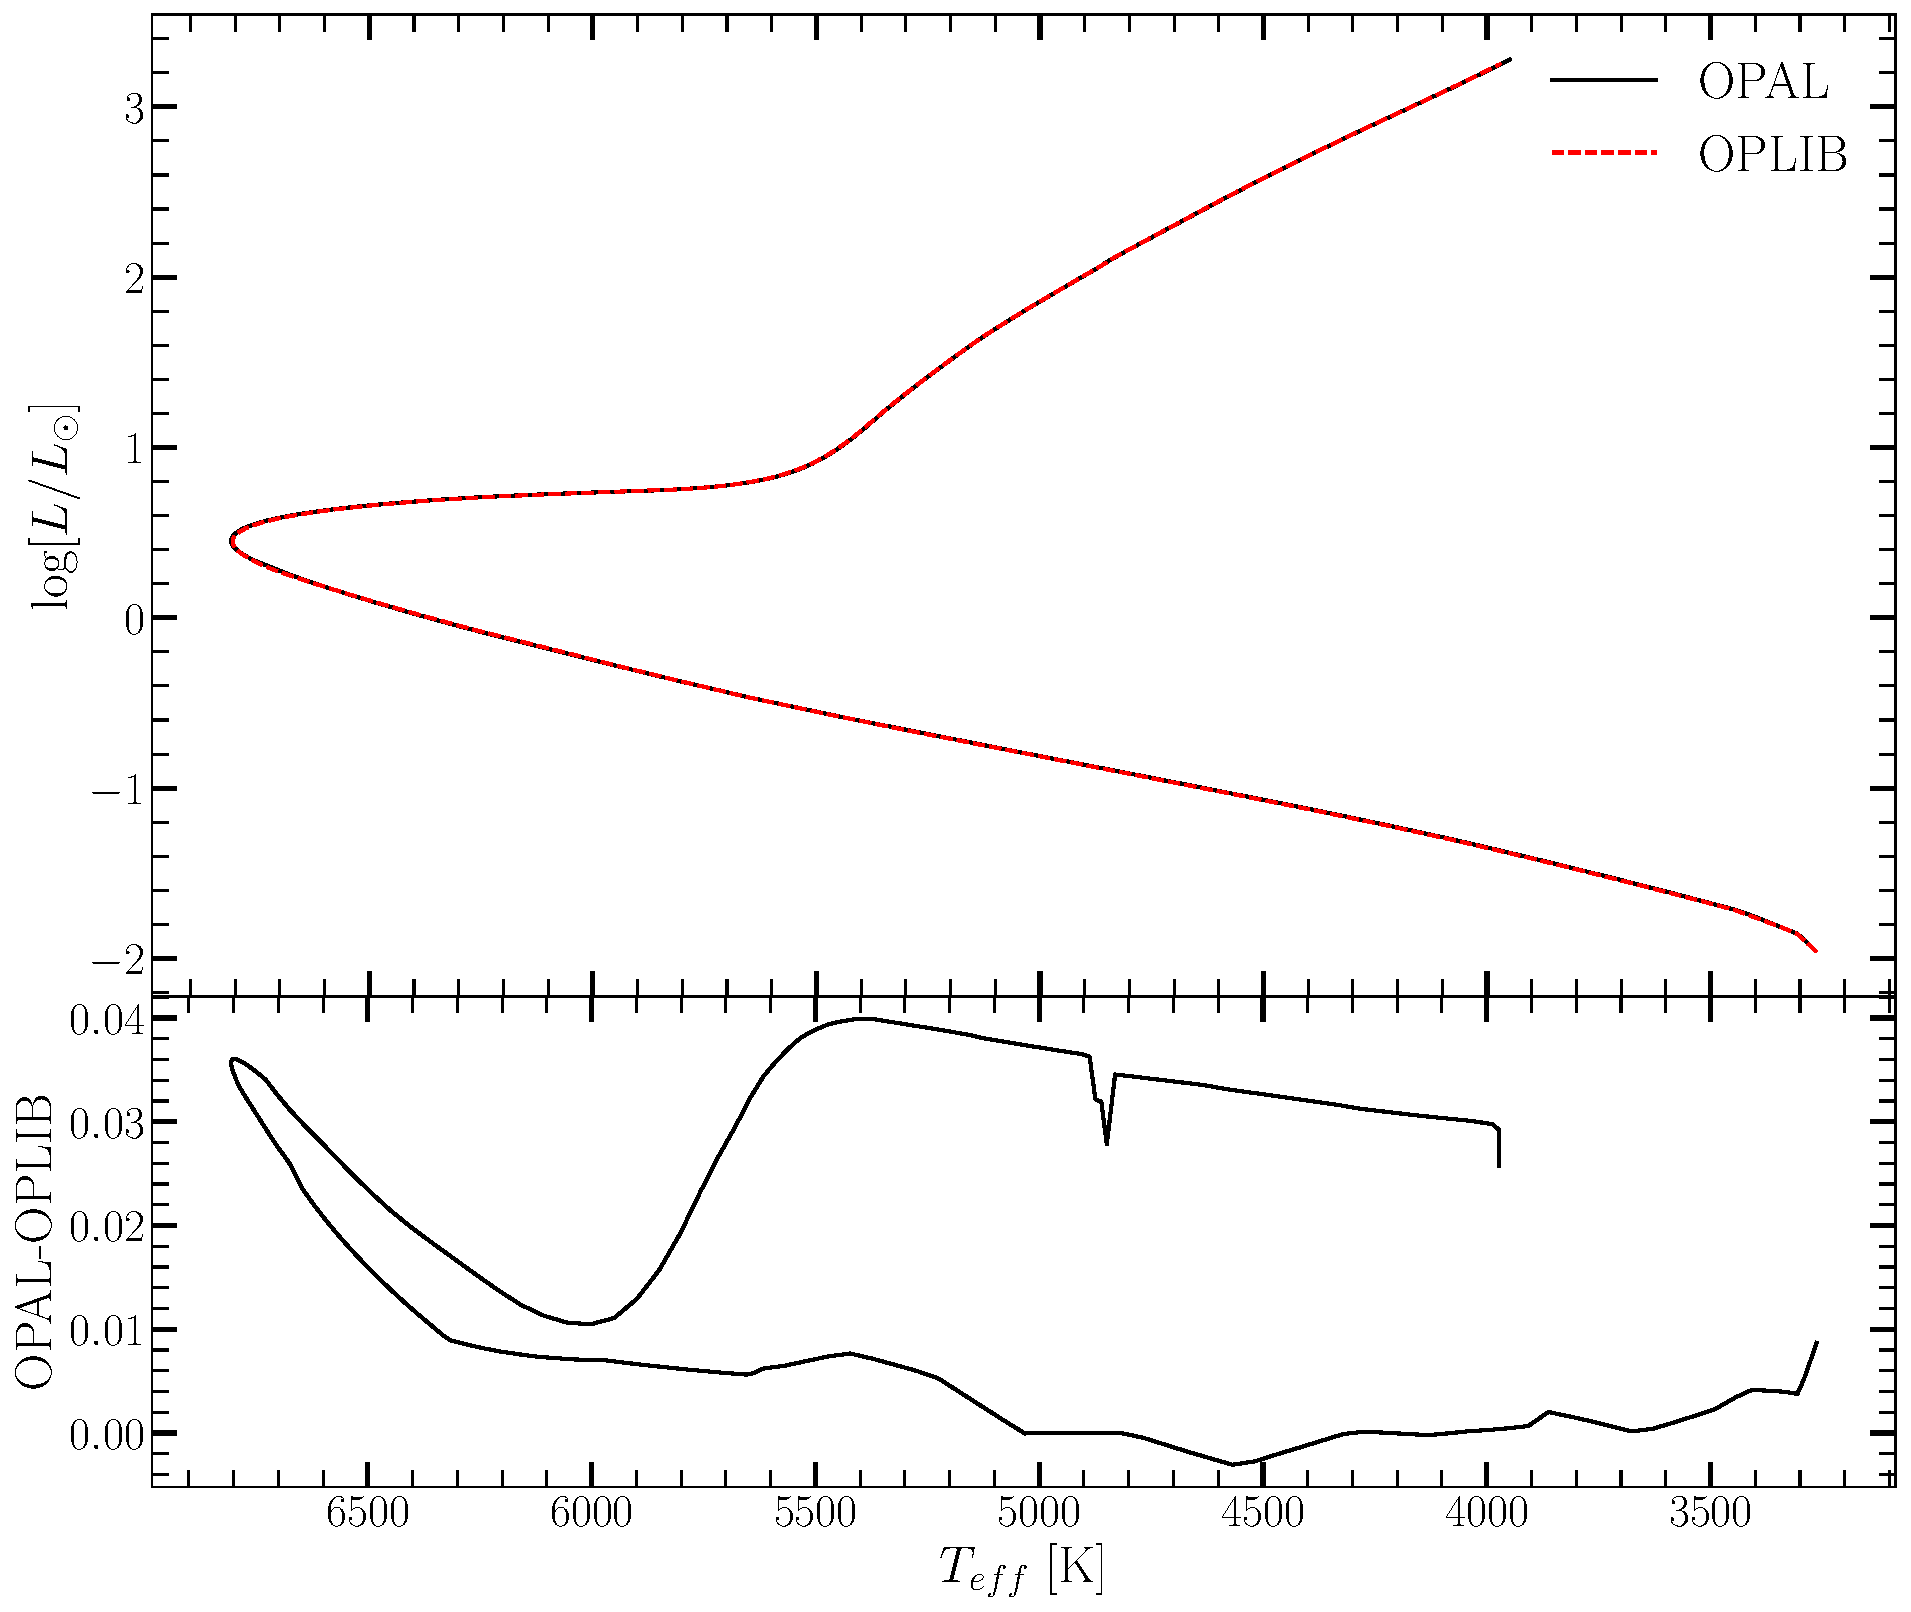
\includegraphics[width=0.45\textwidth]{src/Figures/033ZIsosOPALOPLIB.pdf}
	\caption{10 Gyr \& Y=0.33 isochrones for models generated with OPAL and
	OPLIB opacities tables (top). Residuals between isochrones (bottom).}
	\label{fig:NGC2808ISO}
\end{figure}

\subsubsection{Additional Consistency}
The isochrones used to infer the degree of helium enhancements assume that
convection operates in the same manner in metal-poor stars as it does in the
Sun. However, observations from \textit{Kepler} of metal-poor red giants
\citep{Bonaca2012, tayar2017correlation}, in concert with interferometric
radius determination of the metal-poor sub-giant HD 140283
\citep{creevey2015benchmark}, have shown that the efficiency of convection
changes with iron content. As the final portion of our work to more carefully
handle a stars chemistry, we will modify DSEP to capture this variation in
convective efficiency. 
